\begin{figure}[!b]
    \centering
    \noindent
    \begin{tabular}{cccccc}
        % Montage
        \resizebox{!}{70pt}{
        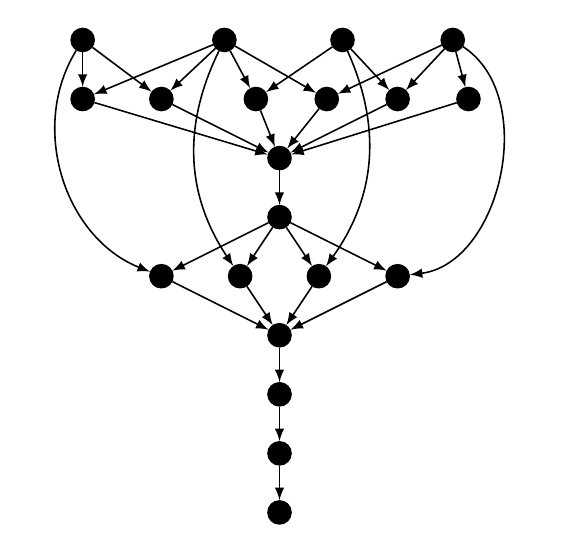
\begin{tikzpicture}
[lineDecorate/.style={-latex,line width=0.2mm}, nodeDecorate/.style={shape=circle,inner sep=3pt,draw}]

 \foreach \nodename/\x/\y in {
0/0/0,
1/1/0,
2/2/0,
3/3/0,
4/1.5/-0.5,
5/1.5/-1.0,
6/1.5/-1.5,
7/1.5/-2,
8/-1/2,
9/0.8/2,
10/2.3/2,
11/3.7/2,
12/-1/1.5,
13/0/1.5,
14/1.2/1.5,
15/2.1/1.5,
16/3/1.5,
17/3.9/1.5,
18/1.5/1.0,
19/1.5/0.5
 }
 {
          \node (T\nodename) at (\x,\y*1.5) [nodeDecorate, fill=black] {};
 }
		
\path
\foreach \startnode/\endnode in {0/4,1/4,2/4,3/4,4/5,5/6,6/7,
8/12,8/13,9/12,9/13,9/14,9/15,10/14,10/16,11/15,11/16,11/17,
12/18,13/18,14/18,15/18,16/18,17/18,
18/19,
19/0,19/1,19/2,19/3}
        {
          (T\startnode) edge[lineDecorate] node {} (T\endnode)
        }

(T8) edge[lineDecorate, bend right=50] node{} (T0)
(T10) edge[lineDecorate, bend left=30] node{} (T2)
(T9) edge[lineDecorate, bend right=30] node{} (T1)
(T11) edge[lineDecorate, bend left=70] node{} (T3);
        \end{tikzpicture}}
         
& 
% Epigenomics
\resizebox{!}{70pt}{
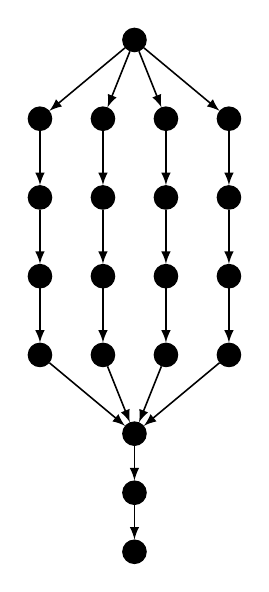
\begin{tikzpicture}
[lineDecorate/.style={-latex,line width=0.2mm}, nodeDecorate/.style={shape=circle,inner sep=3pt,draw}]

 \foreach \nodename/\x/\y in {
0/1.5/0,
1/1.5/-0.5,
2/1.5/-1
 }
 {
          \node (T\nodename) at (\x*0.8,\y*1.5) [nodeDecorate, fill=black] {};
 }
		
		
		 \foreach \x in {0,1,2,3}
 {
          \node (A\x) at (\x*0.8, 4.0) [nodeDecorate, fill=black] {};
		  \node (B\x) at (\x*0.8, 3.0) [nodeDecorate, fill=black] {};
		  \node (C\x) at (\x*0.8, 2.0) [nodeDecorate, fill=black] {};
		  \node (D\x) at (\x*0.8, 1.0) [nodeDecorate, fill=black] {};
 }
 
 \node(H) at (1.5*0.8, 5) [nodeDecorate, fill=black]{};
 
\path
\foreach \startnode/\endnode in {0/1,1/2}
        {
          (T\startnode) edge[lineDecorate] node {} (T\endnode)
        }
\foreach \startnode/\endnode in {H/A1,H/A2,H/A3,H/A0}
        {
          (\startnode) edge[lineDecorate] node {} (\endnode)
 }
 
 \foreach \i in {0,1,2,3}
        {
          (A\i) edge[lineDecorate] node {} (B\i)
		  (B\i) edge[lineDecorate] node {} (C\i)
		  (C\i) edge[lineDecorate] node {} (D\i)
		  (D\i) edge[lineDecorate] node {} (T0)
 };

        
\end{tikzpicture}}

% Inspiral
 \hspace{.2in}\resizebox{!}{70pt}{
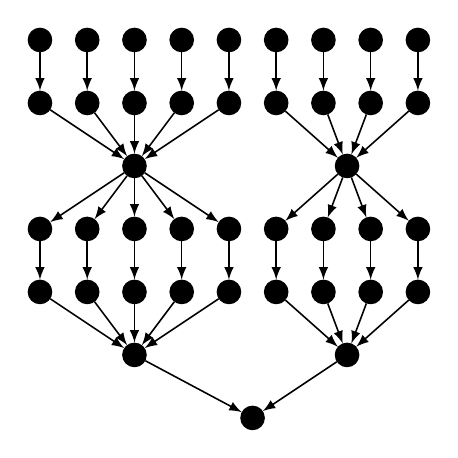
\begin{tikzpicture}
[lineDecorate/.style={-latex,line width=0.2mm}, nodeDecorate/.style={shape=circle,inner sep=3pt,draw}]

 \foreach \i in {0,1,2,3,4,5,6,7,8}
 {
          \node (A\i) at (\i*0.6,5*0.8) [nodeDecorate, fill=black] {};
		  \node (B\i) at (\i*0.6,4*0.8) [nodeDecorate, fill=black] {};
		  \node (E\i) at (\i*0.6,2*0.8) [nodeDecorate, fill=black] {};
		  \node (F\i) at (\i*0.6,1*0.8) [nodeDecorate, fill=black] {};
 }
 \node(C) at (2*0.6,3*0.8) [nodeDecorate, fill=black]{};
 \node(D) at (6.5*0.6,3*0.8) [nodeDecorate, fill=black]{};
 \node(G) at (2*0.6,0*0.8) [nodeDecorate, fill=black]{};
 \node(H) at (6.5*0.6,0*0.8) [nodeDecorate, fill=black]{};
  \node(I) at (4.5*0.6,-1*0.8) [nodeDecorate, fill=black]{};
\path

 \foreach \i in {0,1,2,3,4,5,6,7,8}
        {
          (A\i) edge[lineDecorate] node {} (B\i)
		  (E\i) edge[lineDecorate] node {} (F\i)
 }
  \foreach \i in {0,1,2,3,4}
        {
          (B\i) edge[lineDecorate] node {} (C)
		  (C) edge[lineDecorate] node {} (E\i)
		  (F\i) edge[lineDecorate] node {} (G)
 }
  \foreach \i in {5,6,7,8}
        {
          (B\i) edge[lineDecorate] node {} (D)
		  (D) edge[lineDecorate] node {} (E\i)
		  (F\i) edge[lineDecorate] node {} (H)
 }

 (G) edge[lineDecorate] node {} (I)
 (H) edge[lineDecorate] node {} (I);
\end{tikzpicture}}


\\
~\\

% CyberSkake
\resizebox{!}{50pt}{
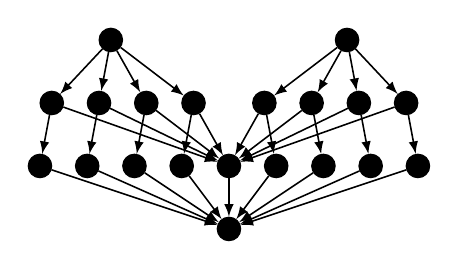
\begin{tikzpicture}
[lineDecorate/.style={-latex,line width=0.2mm}, nodeDecorate/.style={shape=circle,inner sep=3pt,draw}]

 \foreach \i in {0,1,2,3}
 {
          \node (A\i) at (\i*0.6+0.15,1*0.8) [nodeDecorate, fill=black] {};
		  \node (B\i) at (\i*0.6,0*0.8) [nodeDecorate, fill=black] {};
		  
 }
 
  \foreach \i in {5,6,7,8}
 {
          \node (A\i) at (\i*0.6-0.15,1*0.8) [nodeDecorate, fill=black] {};
		  \node (B\i) at (\i*0.6,0*0.8) [nodeDecorate, fill=black] {};
		  
 }
 
 \node(X) at (1.5*0.6, 2*0.8) [nodeDecorate, fill=black]{};
 \node(Y) at (6.5*0.6, 2*0.8) [nodeDecorate, fill=black]{};
\node(K) at (4*0.6, 0*0.8) [nodeDecorate, fill=black]{};
\node(E) at (4*0.6,-1*0.8) [nodeDecorate, fill=black]{};
\path

 \foreach \i in {0,1,2,3}
        {
          (A\i) edge[lineDecorate] node {} (B\i)
		  (A\i) edge[lineDecorate] node {} (K)
		  (B\i) edge[lineDecorate] node {} (E)
		  (X) edge[lineDecorate] node {} (A\i)
 }
 (K) edge[lineDecorate] node{}(E)
  \foreach \i in {5,6,7,8}
        {
          (A\i) edge[lineDecorate] node {} (B\i)
		  (A\i) edge[lineDecorate] node {} (K)
		  (Y) edge[lineDecorate] node {} (A\i)
		  (B\i) edge[lineDecorate] node {} (E)
 };
 
\end{tikzpicture}}


&

% Sipht
\resizebox{!}{50pt}{
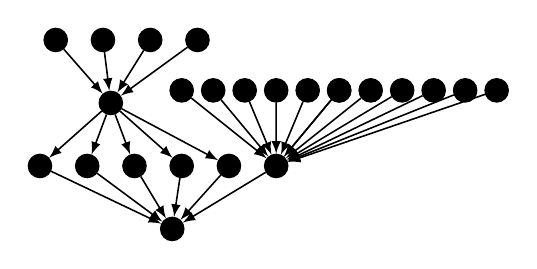
\begin{tikzpicture}
[lineDecorate/.style={-latex,line width=0.2mm}, nodeDecorate/.style={shape=circle,inner sep=3pt,draw}]

 \foreach \i in {0,1,2,3,4}
 {
          \node (A\i) at (\i*0.6,-1*0.8) [nodeDecorate, fill=black] {};
		  
 }
 
  \foreach \i in {0,1,2,3}
 {
          \node (C\i) at (\i*0.6+0.2,1*0.8) [nodeDecorate, fill=black] {};
		  
 }
 
   \foreach \i in {0,1,2,3,4,5,5,6,7,8,9,10}
 {
          \node (F\i) at (\i*0.4+1.8,0.2*0.8) [nodeDecorate, fill=black] {};
		  
 }
 
 \node(B) at (1.5*0.6, 0*0.8) [nodeDecorate, fill=black]{};
 \node(D) at (2.8*0.6, -2*0.8) [nodeDecorate, fill=black]{};
  \node(E) at (5*0.6, -1*0.8) [nodeDecorate, fill=black]{};
\path
(E) edge[lineDecorate] node {} (D)  
 \foreach \i in {0,1,2,3}
        {
          (C\i) edge[lineDecorate] node {} (B)  
 }
  \foreach \i in {0,1,2,3,4}
        {
          (A\i) edge[lineDecorate] node {} (D)
		  (B) edge[lineDecorate] node {} (A\i)
 }
   \foreach \i in {0,1,2,3,4,5,5,6,7,8,9,10}
        {
          (F\i) edge[lineDecorate] node {} (E)
 };
\end{tikzpicture}}



\\
    \end{tabular}
    \caption{
    Some  of  cloud computing  workflows. Clockwise from top left: {\tt Montage, Epigenomics, Inspiral, CyberShake, Sipht}. Each node is one ``task''
    and each edge is a data flow from one task to another.   Number of tasks  can vary from dozens to   thousands).  The configuration problem is to map these tasks to a smaller number
    of virtual machine instances, decide the ordering of tasks within one instance, and
    then decide what kind of machine should drive each instance. For description  of these workflows, see Table~\ref{tab:workflows}.
    }
    \label{fig:structure}
\end{figure}